\documentclass[12pt,addpoints]{evalua}
\grado{2$^\circ$ de Secundaria}
\cicloescolar{2023-2024}
\materia{Ciencias y Tecnología: Física}
\unidad{1}
\title{Examen de la Unidad}
\aprendizajes{\scriptsize%
\item Describe problemas comunes de la vida cotidiana explicando cómo se procede para buscarles solución; conoce y caracteriza el pensamiento científico para plantearse y resolver problemas en la escuela y su cotidianidad.\\[-1.5em]
\item Identifica las unidades de medición que se ocupan en su entorno escolar, familiar y en su comunidad.\\[-1.5em]
\item Relaciona e interpreta las teorías sobre estructura de la materia, a partir de los modelos atómicos y de partículas y los fenómenos que les dieron origen.\\[-1.5em]
\item Experimenta e interpreta los modelos atómicos y de partículas al proponer hipótesis que expliquen los tres estados de la materia, sus propiedades físicas como la temperatura de fusión, ebullición, densidad, entre otros.\\[-1.5em]
}
\author{Prof.: Julio César Melchor Pinto}
\begin{document}
\begin{questions}
      \question[5] Coloca los conceptos en el lugar que les corresponda en la imagen.

      \begin{minipage}[t][][b]{.26\textwidth}\Large
            \wordpill{Sublimación} \wordpill{Fusión} \wordpill{Ebullición} \wordpill{Gaseoso} \wordpill{Sólido} \wordpill{Solidificación} \wordpill{Deposición} \wordpill{Líquido} \wordpill{Condensación}
      \end{minipage}\hfill%
      \begin{minipage}[t][][b]{.6\textwidth}
            \ifprintanswers{
                  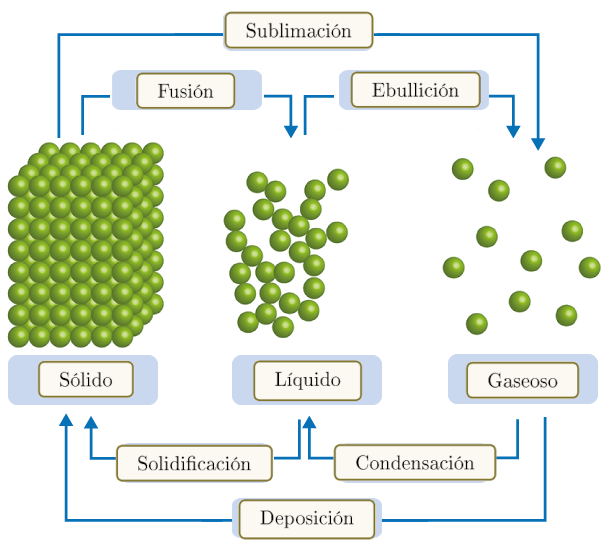
\includegraphics[width=\linewidth]{../images/SINFI_U2_AC47_IMG1_SOL.png}
            }\else{
                  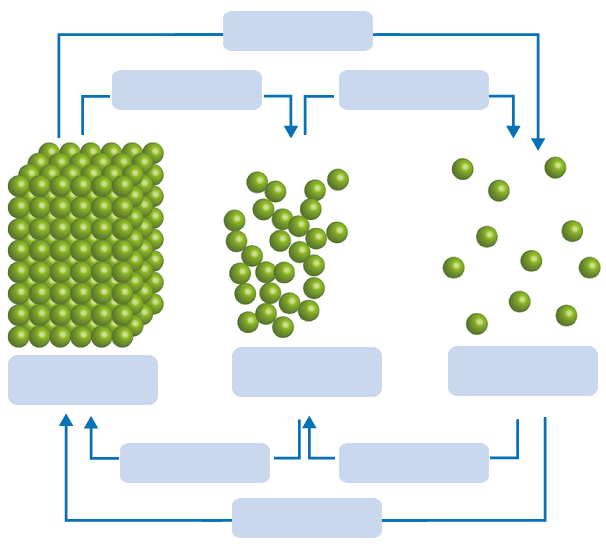
\includegraphics[width=\linewidth]{../images/SINFI_U2_AC47_IMG1.png}
            }\fi
      \end{minipage}

      \begin{minipage}[t][][t]{.4\textwidth}
            \question[10] Ordena los pasos del método científico.\\

            \begin{parts}
                  \part \fillin[5][0.5in] Análisis de resultados
                  \part \fillin[4][0.5in] Experimentación
                  \part \fillin[7][0.5in] Comunicación de resultados
                  \part \fillin[9][0.5in] Teoría científica
                  \part \fillin[1][0.5in] Observación
                  \part \fillin[8][0.5in] Ley científica
                  \part \fillin[2][0.5in] Planteamiento del problema
                  \part \fillin[6][0.5in] Verificación de la hipótesis
                  \part \fillin[3][0.5in] Hipótesis
            \end{parts}
      \end{minipage}\hfill%
      \begin{minipage}[t][][t]{.5\textwidth}
            \question[10] Relaciona las magnitudes físicas fundamentales con su unidad de medida en el Sistema Internacional.

            \setlength{\columnsep}{-1.5em}
            \begin{multicols}{2}
                  \raggedleft \dashedbox{\sffamily\large Cantidades Físicas} \\[1em]

                  \begin{parts}\raggedleft
                        \part Intensidad de la luz  \fillin[F][0.15in]
                        \part Masa                  \fillin[C][0.15in]
                        \part Cantidad de sustancia \fillin[G][0.15in]
                        \part Tiempo                \fillin[A][0.15in]
                        \part Corriente eléctrica   \fillin[D][0.15in]
                        \part Longitud              \fillin[E][0.15in]
                        \part Temperatura           \fillin[B][0.15in]
                  \end{parts}

                  \columnbreak

                  \raggedright  \qquad\dashedbox{\sffamily\large Unidades SI} \\[1.5em]

                  \begin{choices}
                        \choice Segundo
                        \choice Kelvin
                        \choice Kilogramo
                        \choice Ampere
                        \choice Metro
                        \choice Candela
                        \choice Mol
                  \end{choices}

            \end{multicols}
      \end{minipage}

      \question[15] Señala si son \textit{verdaderas} o \textit{falsas} las siguientes frases:
      \begin{multicols}{2}
            \begin{parts}
                  \part El conocimiento empírico se obtiene a través del método científico y la experimentación controlada.

                  \begin{oneparchoices}
                        \choice Verdadero \CorrectChoice Falso
                  \end{oneparchoices}

                  \part El conocimiento empírico es subjetivo y puede variar entre diferentes individuos.

                  \begin{oneparchoices}
                        \CorrectChoice Verdadero \choice Falso
                  \end{oneparchoices}

                  \part El conocimiento empírico usa el razonamiento lógico.

                  \begin{oneparchoices}
                        \choice Verdadero \CorrectChoice Falso
                  \end{oneparchoices}

                  \part El conocimiento empírico puede estar sujeto a preferencias personales y limitaciones sensoriales.

                  \begin{oneparchoices}
                        \CorrectChoice Verdadero \choice Falso
                  \end{oneparchoices}

                  \part El conocimiento empírico siempre es preciso y objetivo.

                  \begin{oneparchoices}
                        \choice Verdadero \CorrectChoice Falso
                  \end{oneparchoices}

                  \part La base del conocimiento empírico se basa en las experiencias del individuo.

                  \begin{oneparchoices}
                        \CorrectChoice Verdadero \choice Falso
                  \end{oneparchoices}

                  \part Las unidades derivadas resultan de combinar dos o más unidades fundamentales.

                  \begin{oneparchoices}
                        \choice Verdadero \CorrectChoice Falso
                  \end{oneparchoices}

                  \part Los grados Celsius son una unidad fundamental.

                  \begin{oneparchoices}
                        \CorrectChoice Verdadero \choice Falso
                  \end{oneparchoices}

                  \part Para medir la velocidad se combinan unidades de distancia y de tiempo.

                  \begin{oneparchoices}
                        \choice Verdadero \CorrectChoice Falso
                  \end{oneparchoices}

                  \part El área combina tres veces las unidades de longitud, como los metros cúbicos.

                  \begin{oneparchoices}
                        \CorrectChoice Verdadero \choice Falso
                  \end{oneparchoices}

                  \part Los newtons son una unidad derivada.

                  \begin{oneparchoices}
                        \CorrectChoice Verdadero \choice Falso
                  \end{oneparchoices}



                  \part El milímetro es un múltiplo del metro

                  \begin{oneparchoices}
                        \CorrectChoice Verdadero \choice Falso
                  \end{oneparchoices}

                  \part El kilogramo es un múltiplo del gramo.

                  \begin{oneparchoices}
                        \CorrectChoice Verdadero \choice Falso
                  \end{oneparchoices}

                  \part Los múltiplos del segundo se utilizan para medir tiempos muy pequeños.

                  \begin{oneparchoices}
                        \CorrectChoice Verdadero \choice Falso
                  \end{oneparchoices}

                  \part Los múltiplos del metro se utilizan para medir distancias y longitudes muy grandes.

                  \begin{oneparchoices}
                        \CorrectChoice Verdadero \choice Falso
                  \end{oneparchoices}
            \end{parts}
      \end{multicols}

      \question[20] Elige la respuesta correcta.
      \begin{multicols}{2}
            \begin{parts}
                  \part Propuesta de una posible explicación del fenómeno.

                  \begin{choices}
                        \choice Observación
                        \choice Teoría científica
                        \choice Experimentación
                        \CorrectChoice Hipótesis
                  \end{choices}

                  \part Se trata de demostrar si la hipótesis es o no correcta mediante un experimento controlado.

                  \begin{choices}
                        \choice Hipótesis
                        \choice Observación
                        \choice Teoría científica
                        \CorrectChoice Experimentación
                  \end{choices}

                  % \part Indica con claridad el problema que se quiere resolver. Delimita y especifica el objeto de su investigación.

                  % \begin{choices}
                  %       \choice Experimentación
                  %       \CorrectChoice Planteamiento del problema
                  %       \choice Ley científica
                  %       \choice Comunicación de resultados
                  % \end{choices}

                  % \part Indica la regularidad que existe en un fenómeno, entre sus causas y sus efectos, normalmente se expresa de manera matemática.

                  % \begin{choices}
                  %       \choice Hipótesis
                  %       \CorrectChoice Ley científica
                  %       \choice Teoría científica
                  %       \choice Experimentación
                  % \end{choices}

                  % \part Si no se comprueba la hipótesis, se plantea una nueva, considerando los datos y la información obtenida en el experimento.

                  % \begin{choices}
                  %       \CorrectChoice Verificación de la hipótesis
                  %       \choice Análisis de resultados
                  %       \choice Teoría científica
                  %       \choice Comunicación de resultados
                  % \end{choices}

                  % \part El científico observa la realidad que le rodea, aísla el fenómeno que le interesa e identifica las variables que intervienen.

                  % \begin{choices}
                  %       \choice Hipótesis
                  %       \CorrectChoice Observación
                  %       \choice Teoría científica
                  %       \choice Verificación de la hipótesis
                  % \end{choices}



                  \part La hipótesis se confirma o se rechaza analizando los datos y la información obtenida en los experimentos.

                  \begin{choices}
                        \choice Ley científica
                        \CorrectChoice Análisis de resultados
                        \choice Experimentación
                        \choice Observación
                  \end{choices}

                  \part Explicación de un fenómeno a partir de leyes científicas.

                  \begin{choices}
                        \CorrectChoice Teoría científica
                        \choice Ley científica
                        \choice Análisis de resultados
                        \choice Comunicación de resultados
                  \end{choices}

                  \part El científico comparte los resultados de su investigación a la comunidad científica mediante tesis, artículos científicos o congresos.

                  \begin{choices}
                        \CorrectChoice Comunicación de resultados
                        \choice Ley científica
                        \choice Análisis de resultados
                        \choice Teoría científica
                  \end{choices}

                  \part Son materiales que permiten la conducción de calor y electricidad.

                  \begin{choices}
                        \choice Materiales inorgánicos  \choice Materiales metálicos  \choice Materiales tóxicos  \choice Materiales refractarios
                  \end{choices}

                  \part Son materiales derivados del petróleo y pueden ser moldeados para lograr distintos objetos.

                  \begin{choices}
                        \choice Materiales refractarios  \choice Materiales plásticos  \choice Materiales textiles  \choice Materiales metálicos.
                  \end{choices}

                  \part Es todo aquello que ocupa un lugar en espacio.

                  \begin{choices}
                        \choice Masa  \choice Densidad  \choice Volumen  \CorrectChoice Materia
                  \end{choices}

                  \part Es el espacio que ocupa un objeto.

                  \begin{choices}
                        \choice Masa  \choice Densidad  \CorrectChoice Volumen  \choice Materia
                  \end{choices}

                  \part Es la cantidad de materia que posee un cuerpo.

                  \begin{choices}
                        \CorrectChoice Masa  \choice Densidad  \choice Volumen  \choice Materia
                  \end{choices}
            \end{parts}
      \end{multicols}


      \newpage
      \question[5] Elige la respuesta para cada pregunta.
      \begin{multicols}{2}
            \begin{parts}
                  \part Un corresponsal de noticias informa que las altas temperaturas en California, Estados Unidos, alcanzaron 113 °F. ¿Cuál es la temperatura equivalente en grados centígrados?

                  \begin{oneparchoices}
                        \CorrectChoice 45 °C \choice 55 °C
                  \end{oneparchoices}

                  \part José observa el informe del clima durante un viaje de negocios en Dublín (Irlanda). El conductor de noticias asegura que la temperatura se elevará de los 64.4 °F actuales a 102.2 °F. ¿Cuál es el incremento de temperatura correspondiente en la escala Celsius?

                  \begin{oneparchoices}
                        \CorrectChoice 21 °C \choice 37.8 °C
                  \end{oneparchoices}

                  \part Pedro se siente mal y decide ir al médico, éste le informa que su temperatura corporal es de 313.15 K. Pedro sabe que una persona tiene fiebre cuando su temperatura es superior a 37 °C. ¿Cuál es el estado de salud de Pedro?

                  \begin{oneparchoices}
                        \CorrectChoice Pedro tiene fiebre \choice Pedro no tiene fiebre
                  \end{oneparchoices}

                  \part Mónica cocinará un pavo en Navidad y desea que su familia realmente lo disfrute, por lo que se prepara estudiando un recetario de cocina profesional. En él encuentra que debe precalentar el horno a 325 °F, pero su horno utiliza la escala Celsius. ¿Cuál es la temperatura equivalente?

                  \begin{oneparchoices}
                        \CorrectChoice 100 °C \choice 162.7 °C
                  \end{oneparchoices}

                  \part De compras en un centro comercial, Francisco lee en la etiqueta de una lata de atún: “Mantener por debajo de 296.15 K. ¿Cuál es la temperatura correspondiente en la escala Celsius?

                  \begin{oneparchoices}
                        \CorrectChoice 23 °C \choice 47 °C
                  \end{oneparchoices}

                  \part Mexicali, capital de Baja California, es la ciudad más calurosa de México. Debido a su ubicación de tipo desierto interior, las temperaturas alcanzan 40 °C. ¿A qué temperatura equivale esto en la escala Fahrenheit?

                  \begin{oneparchoices}
                        \CorrectChoice 72 °F \choice 104 °F
                  \end{oneparchoices}

                  \part El cuerpo humano resiste mejor los descensos de temperatura que los aumentos en la misma. Un descenso significativo de temperatura sólo provoca una lentificación de las funciones celulares, mientras que un aumento de la misma magnitud provocaría la pérdida definitiva de tales funciones. La temperatura máxima que puede soportar el cuerpo humano es 316.15 K. ¿A qué temperatura equivale en la escala Celsius y Fahrenheit?

                  \begin{oneparchoices}
                        \choice 109,4 °C y 43 °F \CorrectChoice 43 °C y 109.4 °F
                  \end{oneparchoices}

                  \part El 10 de agosto del 2010, un grupo de investigadores registró en la Antártida la temperatura más baja del planeta: 93 °C bajo cero. ¿Cuál es la temperatura correspondiente en la escala de temperatura absoluta?

                  \begin{oneparchoices}
                        \CorrectChoice 180.15 K \choice 366.15 K
                  \end{oneparchoices}

                  \part Venus no es el planeta más cercano al Sol, pero sí el más caliente, pues posee una atmósfera muy densa que impide que el calor proveniente del Sol escape del planeta (efecto invernadero). Alcanza temperaturas de hasta 864 °F. ¿Cuál es la temperatura correspondiente en la escala Celsius?

                  \begin{oneparchoices}
                        \CorrectChoice 462.22 °C \choice 1587.2 °C
                  \end{oneparchoices}

                  \part Rubén colocó un vaso con agua en el refrigerador y lo dejó ahí hasta que el agua sufrió un descenso de temperatura de 20.3 °C. ¿Cuál es el cambio de temperatura correspondiente en K?

                  \begin{oneparchoices}
                        \choice 20.3 K \CorrectChoice 293.45 K
                  \end{oneparchoices}

                  \part Según la agencia científica de Naciones Unidas, la temperatura promedio en la superficie de la Tierra y de los océanos fue la más alta en el periodo de enero a octubre de 2014, al alcanzar 14.78 °C. ¿Cuál es la temperatura correspondiente en grados Fahrenheit?

                  \begin{oneparchoices}
                        \choice 26.604 °F \CorrectChoice  58.604 °F
                  \end{oneparchoices}

                  \part El punto de fusión del oro es 1 064 °C y la plata se funde a 1 234.93 K. ¿Cuál de los dos tiene una temperatura de fusión más elevada?

                  \begin{oneparchoices}
                        \CorrectChoice El oro \choice La plata
                  \end{oneparchoices}

            \end{parts}
      \end{multicols}



      % \question[5] Elige la respuesta correcta
      % \begin{multicols}{2}
      %       \begin{parts}

      %       \end{parts}
      % \end{multicols}

      \question[5] Coloca los conceptos en el lugar que les corresponda en la imagen.\\

      \begin{center}
            \wordpill{Mecánica estadística}
            \wordpill{Estudia los átomos y su constitución}
            \wordpill{Relatividad}
            \wordpill{Fuerza}
            \wordpill{Describe el movimiento de los objetos}
            \wordpill{Física clásica}
            \wordpill{Física moderna}
            \wordpill{Calor y temperatura}
            \vspace*{1em}
            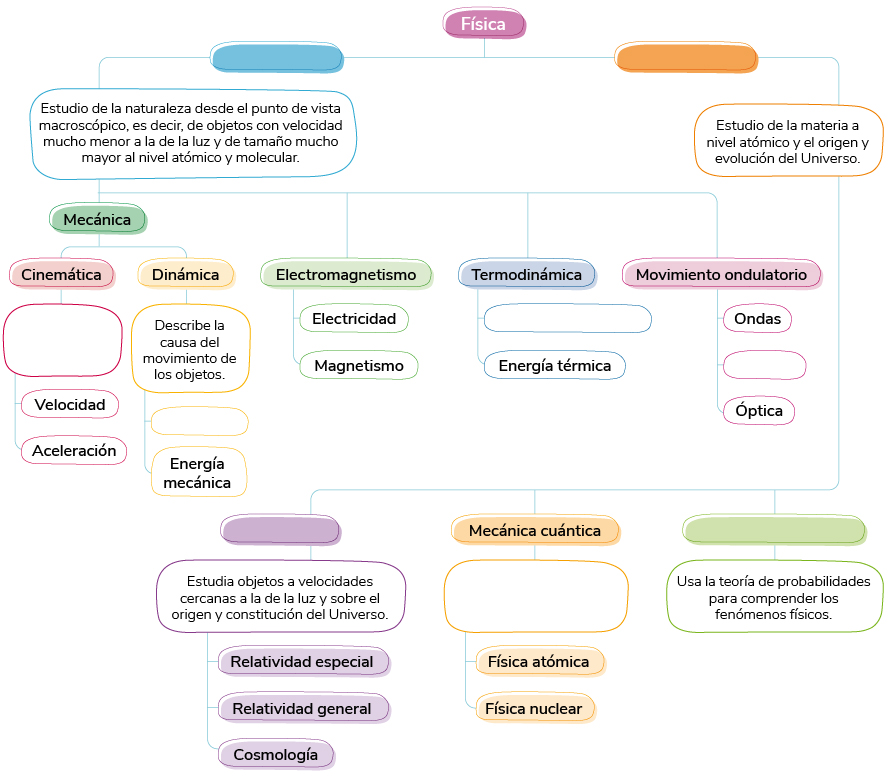
\includegraphics[width=.95\textwidth]{../images/SIM_FI2_SB_U1_P28_IMG01.jpg}
      \end{center}

      \question[5] Relaciona los elementos.
      \begin{multicols}{2}
            \begin{parts}\raggedleft\footnotesize
                  \part Número $50 000$ en notación científica.                                                                                           \fillin[][0.2in]
                  \part Número $0.0000032$ en notación científica.                                                                                        \fillin[][0.2in]
                  \part En notación científica es el número $610 000 000 000$.                                                                            \fillin[][0.2in]
                  \part En notación decimal es el número $7.8 \times 10^{-4}$.                                                                            \fillin[][0.2in]
                  \part Notación decimal del número $9.5 \times 108$.                                                                                     \fillin[][0.2in]
                  \part La masa de una ballena azul es de 150 000 kg. ¿Cuál es el valor en notación científica?                                           \fillin[][0.2in]
                  \part El tamaño de un átomo es una diezmilmillonésima de metro, ¿cómo se escribe este número en notación científica?                    \fillin[][0.2in]
                  \part El diámetro de un cabello es de 80 micrómetros. ¿Cuál es este número con notación científica y en metros?                         \fillin[][0.2in]
                  \part La  masa del Sol es $1.989 \times 1030$ kg, si lo escribieras en notación decimal, ¿cuántos ceros tendrías que agregar al número? \fillin[][0.2in]
                  \part La distancia de la Tierra a Neptuno es de 4345 millones de km, ¿cuál es su número con notación científica y en centímetros?       \fillin[][0.2in]
                  \part ¿Cuántos segundos tarda la Tierra en completar una rotación sobre su eje?                                                         \fillin[][0.2in]
                  \part Neptuno tarda 165 años en completar una vuelta alrededor del Sol, ¿a cuántos minutos equivalen, escrito en notación científica?   \fillin[][0.2in]
                  \part La temperatura de la superficie del Sol es de 5772 K, ¿a cuántos mK equivalen?                                                    \fillin[][0.2in]
                  \part La masa de la Tierra es $5.972 \times 10^{24}$ kg. Si la escribieras en notación decimal, ¿cuántos ceros tienes que agregar?      \fillin[][0.2in]
                  \part La masa promedio de una mosca es de 14 mg, ¿cuál es su valor en gramos?.                                                          \fillin[][0.2in]
            \end{parts}

            \columnbreak

            \begin{choices}
                  \choice $5.772  \times 10^6$ mK
                  \choice $10^{-10}$ m
                  \choice $8 \times 10^{-5}$ m
                  \choice $950 000 000$
                  \choice $8.64 \times 10^4$ s
                  \choice $27$
                  \choice $6.1 \times 10^{11}$
                  \choice $0.00078$
                  \choice $0.014$ g
                  \choice $5 \times 10^4$
                  \choice $21$
                  \choice $4.345 \times 10^{14}$ cm
                  \choice $1.5 \times 10^5$ kg
                  \choice $8.672 \times 10^7$ min
                  \choice $3.2 \times 10^{-6}$
            \end{choices}
      \end{multicols}






      \question[10] Coloca los conceptos en el lugar que les corresponda en la imagen\\

      \begin{minipage}[b][][b]{.2\textwidth}
            \ifprintanswers{
            }\else{
                  \wordpill{Ernest Rutherford}
                  \wordpill{El descubrimiento del electrón}
                  \wordpill{Niels Bohr}
                  \wordpill{Neutrones}
                  \wordpill{Modelo cuántico del átomo}
                  \wordpill{Descubrir el átomo de hidrógeno}
                  \wordpill{Explicar los espectros luminosos}
                  \wordpill{El descubrimiento del núcleo atómico}
                  \wordpill{Modelo atómico del ``panqué con pasas''}

            }\fi
      \end{minipage}\hfill%
      \begin{minipage}[b][][b]{.7\textwidth}
            \ifprintanswers{
                  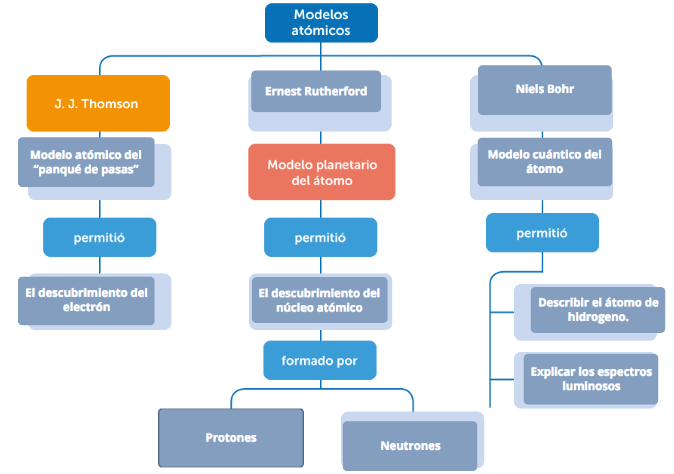
\includegraphics[width=\linewidth]{../images/SINFI_U2_AC65_IMGS1_sol.png}
            }\else{
                  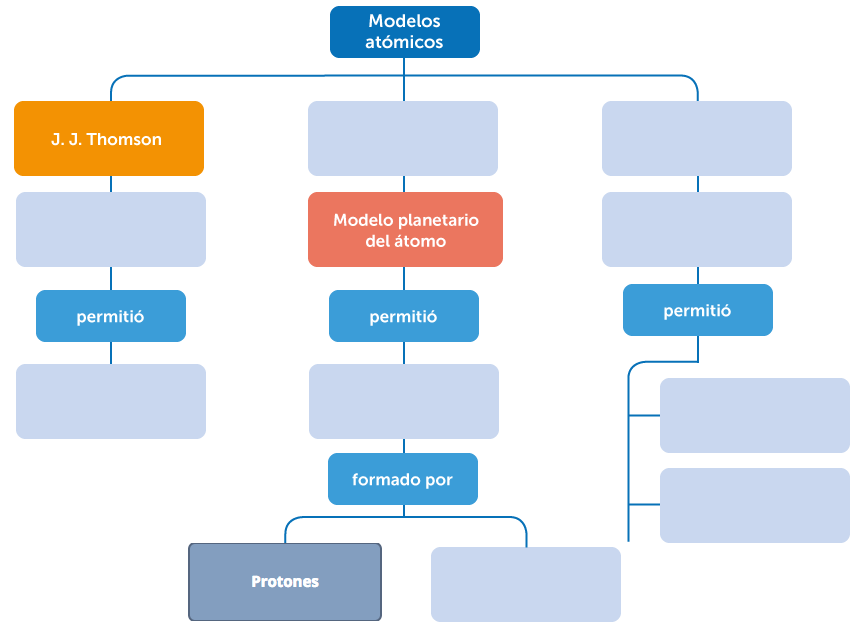
\includegraphics[width=\linewidth]{../images/SINFI_U2_AC65_IMGS1.png}
            }\fi
      \end{minipage}

      % \question[5] Señala si son \textit{verdaderas} o \textit{falsas} las siguientes frases:

      % \begin{multicols}{2}
      %       \begin{parts}
      %             \part Los electrones son partículas tan pequeñas que no es posible observarlas a simple vista, pero podemos saber de ellas a través de fenómenos como la electricidad, los espectros luminosos y el magnetismo.

      %             \begin{oneparchoices}
      %                   \CorrectChoice Verdadero \choice Falso
      %             \end{oneparchoices}

      %             \part Los electrones son partículas de carga negativa cubiertas por una nube de carga positiva; la magnitud de ambas cargas es igual, por lo que son eléctricamente neutros.

      %             \begin{oneparchoices}
      %                   \choice Verdadero \CorrectChoice Falso
      %             \end{oneparchoices}

      %             \part Todos los elementos radiactivos pueden emitir partículas llamadas alfa (carga positiva), beta (carga negativa) y gama (sin carga).

      %             \begin{oneparchoices}
      %                   \CorrectChoice Verdadero \choice Falso
      %             \end{oneparchoices}

      %             \part En su experimento con partículas alfa, Rutherford encontró que algunas de éstas rebotaban después de chocar con la lámina metálica, por lo que concluyó que colisionaban con obstáculos de carga positiva.

      %             \begin{oneparchoices}
      %                   \CorrectChoice Verdadero \choice Falso
      %             \end{oneparchoices}

      %             \part Todos los elementos emiten partículas alfa, que poseen carga positiva; beta, que tienen carga negativa; y rayos gama, que no tienen carga eléctrica.

      %             \begin{oneparchoices}
      %                   \choice Verdadero \CorrectChoice Falso
      %             \end{oneparchoices}

      %             \columnbreak

      %             \part El núcleo está formado por protones, que tienen carga positiva, y neutrones, que no poseen carga (es decir, son eléctricamente neutros).

      %             \begin{oneparchoices}
      %                   \CorrectChoice Verdadero \choice Falso
      %             \end{oneparchoices}

      %             \part Cuando Rutherford colisionó partículas alfa sobre una lámina metálica delgada, encontró que se desviaban muy poco de su trayectoria original, por lo que de inmediato concluyó que el modelo atómico de Thomson era correcto.

      %             \begin{oneparchoices}
      %                   \choice Verdadero \CorrectChoice Falso
      %             \end{oneparchoices}

      %             \part El modelo de Rutherford no pudo explicar por qué aparecían delgadas líneas oscuras entre las franjas de colores del espectro producido por la luz del Sol; este fenómeno sólo encontraría respuesta con el modelo atómico de Niels Bohr.


      %             \begin{oneparchoices}
      %                   \CorrectChoice Verdadero \choice Falso
      %             \end{oneparchoices}

      %             \part Si los átomos estuvieran formados sólo por electrones, cualquier objeto estaría cargado negativamente y su electricidad sería evidente.

      %             \begin{oneparchoices}
      %                   \CorrectChoice Verdadero \choice Falso
      %             \end{oneparchoices}
      %       \end{parts}
      % \end{multicols}



      \question[5] Señala si los siguientes procesos son \textit{físicos} o \textit{químicos}.
      \begin{multicols}{2}
            \begin{parts}
                  \part Romper una hoja de papel.

                  \begin{oneparchoices}
                        \CorrectChoice Físico \choice Químico
                  \end{oneparchoices}

                  \part Digerir y absorber los alimentos.

                  \begin{oneparchoices}
                        \choice Físico \CorrectChoice Químico
                  \end{oneparchoices}

                  \part Derretir una vela.

                  \begin{oneparchoices}
                        \CorrectChoice Físico \choice Químico
                  \end{oneparchoices}

                  \part Encender fuegos artificiales.

                  \begin{oneparchoices}
                        \choice Físico \CorrectChoice Químico
                  \end{oneparchoices}

                  \part Hornear un pastel de vainilla.

                  \begin{oneparchoices}
                        \choice Físico \CorrectChoice Químico
                  \end{oneparchoices}

                  \part Apretar una lata de aluminio.

                  \begin{oneparchoices}
                        \CorrectChoice Físico \choice Químico
                  \end{oneparchoices}

                  \part Derretir un cubo de hielo.

                  \begin{oneparchoices}
                        \CorrectChoice Físico \choice Químico
                  \end{oneparchoices}

                  \part Cocinar un huevo estrellado.

                  \begin{oneparchoices}
                        \choice Físico \CorrectChoice Químico
                  \end{oneparchoices}
            \end{parts}
      \end{multicols}

\end{questions}
\end{document}